%%%%%%%%%%%%%%%%%%%%%%%%%%%%%%%%%%%%%%%%
%
% $ Autor: Gruppe 07 $
% $ Projekt: Magic Faucet Fountain $
% $ Pfad: LaTeXTemplate/Montageanleitung/Chapters/de/LetzteSchritte.tex $
% $ Kurzbeschreibung: Dieses Dokument erstellt den Abschluss der Montageanleitung $
%
% !TeX spellcheck = de_DE/GB
% !TeX program = pdflatex
% !BIB program = biber/bibtex
% !TeX encoding = utf8
%
%%%%%%%%%%%%%%%%%%%%%%%%%%%%%%%%%%%%%%%%

\chapter{Abschluss}
\begin{center}
	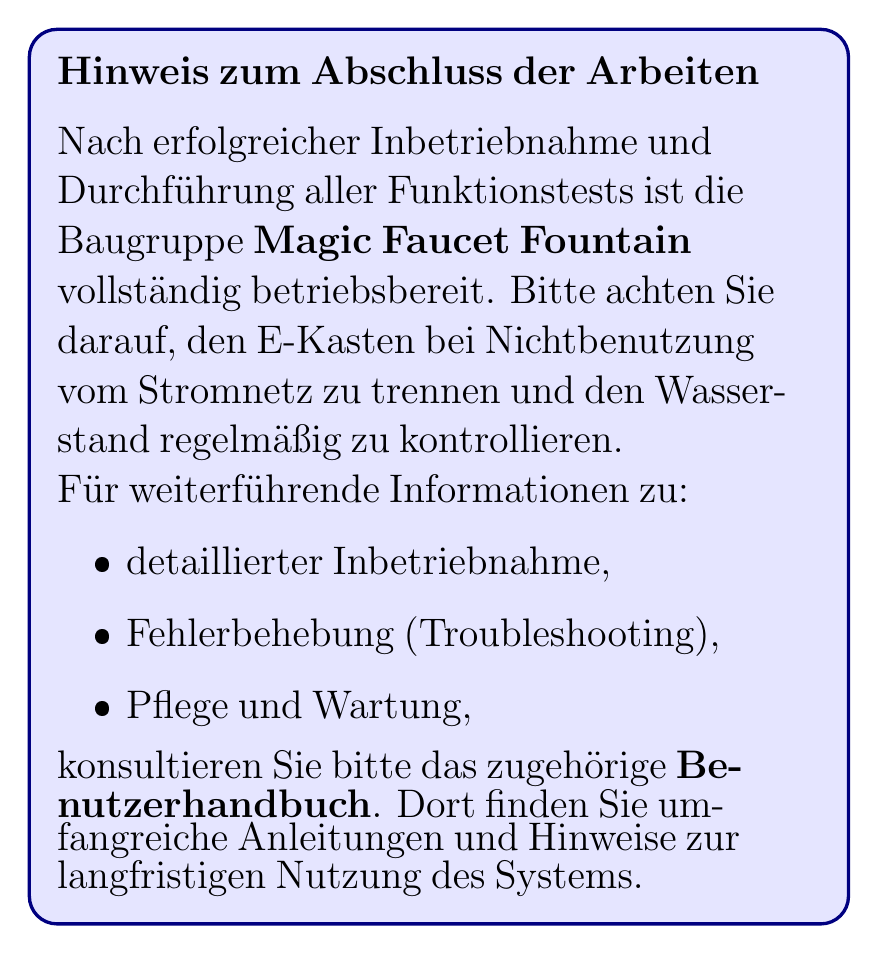
\begin{tikzpicture}
		\node[rectangle, draw=blue!50!black, very thick, fill=blue!10, rounded corners=10pt, inner sep=10pt, text width=0.8\textwidth] (box) {
			\Large \textbf{Hinweis zum Abschluss der Arbeiten}
			
			\vspace{0.5em}
			
			Nach erfolgreicher Inbetriebnahme und Durchführung aller Funktionstests ist die Baugruppe \textbf{Magic Faucet Fountain} vollständig betriebsbereit. Bitte achten Sie darauf, den E-Kasten bei Nichtbenutzung vom Stromnetz zu trennen und den Wasserstand regelmäßig zu kontrollieren.
			
			Für weiterführende Informationen zu:
			\begin{itemize}
				\item detaillierter Inbetriebnahme,
				\item Fehlerbehebung (Troubleshooting),
				\item Pflege und Wartung,
			\end{itemize}
			konsultieren Sie bitte das zugehörige \textbf{Benutzerhandbuch}. Dort finden Sie umfangreiche Anleitungen und Hinweise zur langfristigen Nutzung des Systems.
		};
	\end{tikzpicture}
\end{center}


